\documentclass[12pt,spanish]{article}
\usepackage[spanish]{babel}
\usepackage{graphicx}
\usepackage{color}
\usepackage{xcolor}
\usepackage{colortbl}
\usepackage{amsthm,thmtools}
\usepackage{dirtytalk}
\usepackage{multirow}
\usepackage{amsmath}
\usepackage{subcaption}
\usepackage{adjustbox}
\usepackage{amsmath}
\usepackage{centernot}
\usepackage{mathtools}
\usepackage{multirow}
\usepackage[hidelinks]{hyperref}
\usepackage{caption}
\usepackage{eurosym} % para el euro
\usepackage{amsthm}
\usepackage{multicol}
\usepackage{float}
\usepackage{amsfonts}
\usepackage{titling}
\usepackage{soul}
\usepackage{listings}
\usepackage{array}
\usepackage{tikz}
\usetikzlibrary{shapes.geometric, arrows, chains, calc,positioning,fit,decorations.pathreplacing}
\usepackage[framemethod=tikz]{mdframed}

\graphicspath{ {../img/}}
\selectlanguage{spanish}
\usepackage[utf8]{inputenc}
\usepackage{graphicx}
\usepackage[a4paper,left=3cm,right=2cm,top=2.5cm,bottom=2.5cm]{geometry}

\newenvironment{solution}{
	\par
	\textbf{Solución}
	\par
	\begin{center}
}
{
	\end{center}
}

\lstset{
  breaklines=true,
  postbreak=\mbox{\textcolor{red}{$\hookrightarrow$}\space},
}


\title{Servidores Web de Altas Prestaciones}
\setlength{\droptitle}{10em}
\author{Carlos Sánchez Páez}

\makeindex
\begin{document}
\definecolor{light-gray}{gray}{0.95}
\lstset{columns=fullflexible,basicstyle=\ttfamily}
\surroundwithmdframed[
  hidealllines=true,
  backgroundcolor=light-gray,
  innerleftmargin=0pt,
  innertopmargin=0pt,
  innerbottommargin=0pt]{lstlisting}


\begin{titlepage}

 \newlength{\centeroffset}
 \setlength{\centeroffset}{-0.5\oddsidemargin}
 \addtolength{\centeroffset}{0.5\evensidemargin}
 \thispagestyle{empty}

 \noindent\hspace*{\centeroffset}
 \begin{minipage}{\textwidth}

  \centering
  
\includegraphics[width=0.9\textwidth]{logo_ugr.jpg}\\[1.4cm]

  \textsc{ \Large Servidores Web de Altas Prestaciones\\[0.2cm]}
  \textsc{GRADO EN INGENIERÍA INFORMÁTICA}\\[1cm]

  {\Huge\bfseries Prácticas resueltas \\}
 \end{minipage}

 \vspace{1.5cm}
 \noindent\hspace*{\centeroffset}
 \begin{minipage}{\textwidth}
  \centering

  \textbf{Autor}\\ {Carlos Sánchez Páez}\\[2.5ex]
  
\includegraphics[width=0.4\textwidth]{etsiit_logo.png}\\[0.1cm]
  \vspace{1.5cm}
  
\includegraphics[width=0.15\textwidth]{atc.jpg}\\[0.1cm]
  \vspace{1cm}
  \textsc{Escuela Técnica Superior de Ingenierías Informática y de Telecomunicación}\\
  \vspace{1cm}
  \textsc{Curso 2019-2020}
 \end{minipage}
\end{titlepage}
\thispagestyle{empty}
\newpage
\tableofcontents{}
\newpage
\listoffigures
\thispagestyle{empty}
\newpage

\section{Práctica 1}

En esta práctica configuraremos dos máquinas virtuales (\textit{M1} y \textit{M2}). También crearemos una interfaz \emph{host-only} para que las máquinas puedan conectarse entre ellas. \\

En esta guía configuraremos la interfaz sólo anfitrión manualmente en una máquina. En la otra dejaremos que el asistente de instalación lo haga por nosotros.

\begin{enumerate}
	\item Comenzaremos creando las máquinas virtuales desde VirtualBox. Las proveeremos de al menos 512MB de RAM y 10GB de disco duro.
	\item Descargamos la imagen ISO de Ubuntu Server 18.04 y la montamos en la unidad de disco de la primera máquina.
	\item Arrancamos la máquina e iniciamos el asistente de instalación. Establecemos nuestro nombre de usuario de GitHub como \emph{username} y \emph{m1} como nombre del servidor. La clave será \emph{Swap1234}
	\item Cuando termine la instalación apagamos la máquina.
	\item En VirtualBox abrimos el administrador de redes sólo antitrión (dentro del menú Archivo).
	\item Creamos un adaptador y activamos DHCP para que asigne una IP a nuestra máquina.
	\begin{figure}[H]
		\centering
		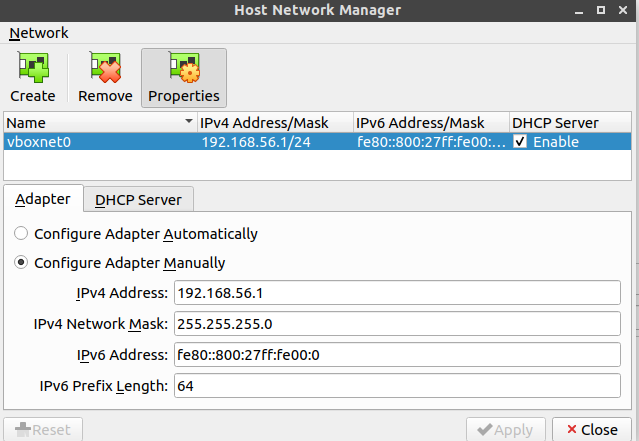
\includegraphics[scale=0.65]{/p1/host_only.png}
	\end{figure}
	\item Vamos a los ajustes de red de la máquina y "conectamos" el adaptador que acabamos de crear.
	\begin{figure}[H]
		\centering
		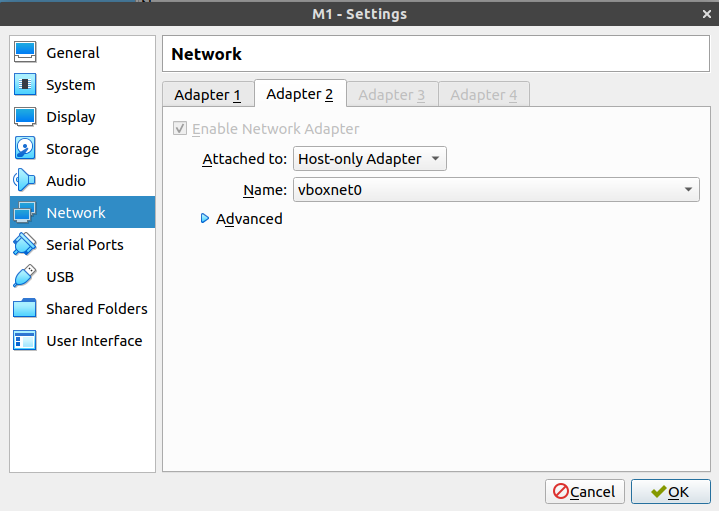
\includegraphics[scale=0.65]{/p1/host_only_2.png}
	\end{figure}
	\item Arrancamos la máquina. Ejecutamos el siguiente comando para ver las interfaces conectadas:
	\begin{lstlisting}
		m1> sudo ifconfig -a
	\end{lstlisting}
	\begin{figure}[H]
		\centering
		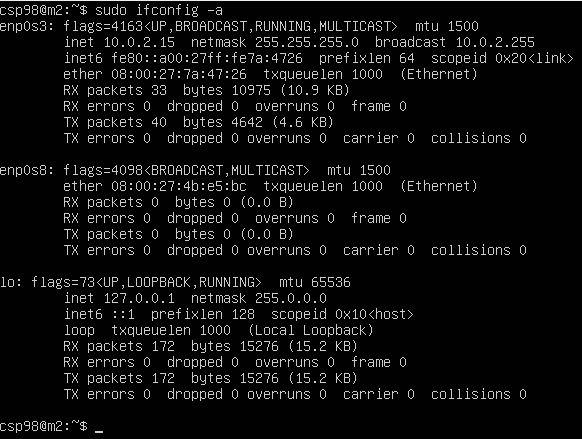
\includegraphics[scale=0.65]{/p1/ifconfig_noip.png}
	\end{figure}
	\item Vemos que tenemos una nueva interfaz (\emph{enp0s8}) pero no tiene IP asignada. Para arreglar esto usaremos \emph{netplan}.
	\item Creamos un archivo de configuración para ella:
	\begin{lstlisting}
		m1> sudo nano /etc/netplan/host-only.yaml
	\end{lstlisting}
	\item Introducimos este contenido en el archivo. Debemos usar espacios en vez de tabuladores.
	\begin{lstlisting}
		network:
		  version: 2
			renderer: networkd
			ethernets:
			  enp0s8:
				  dhcp4: true
	\end{lstlisting}
	\item Guardamos los cambios y los aplicamos con el comando
	\begin{lstlisting}
		m1> sudo netplan apply
	\end{lstlisting}
	\item Ejecutamos \emph{sudo ifconfig -a} y comprobamos que ya tenemos IP asignada:
	\begin{figure}[H]
		\centering
		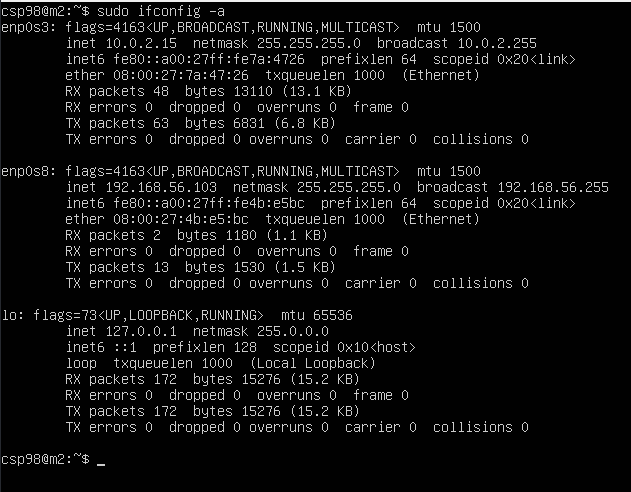
\includegraphics[scale=0.65]{/p1/ifconfig.png}
	\end{figure}
	\item Instalamos la pila LAMP:
	\begin{lstlisting}
	m1> sudo apt install -y openssh-server openssh-client apache2 mysql-server mysql-client
	\end{lstlisting}
	\item Pasamos ahora a la configuración de \emph{m2}. Para ello seguimos los pasos anteriores. Como el adaptador sólo anfitrión ya está creado, el asistente de instalación lo configurará automáticamente. Lo único que tenemos que hacer es "conectarlo" a la máquina como hicimos antes.
	\item Cuando termine la instalación, ejecutamos el comando anterior para instalar la pila LAMP.
	\item Probamos la conexión SSH conectando las máquinas entre sí. Para facilitar las conexiones podemos guardar las IPs en variables:
	\begin{figure}[H]
		\centering
		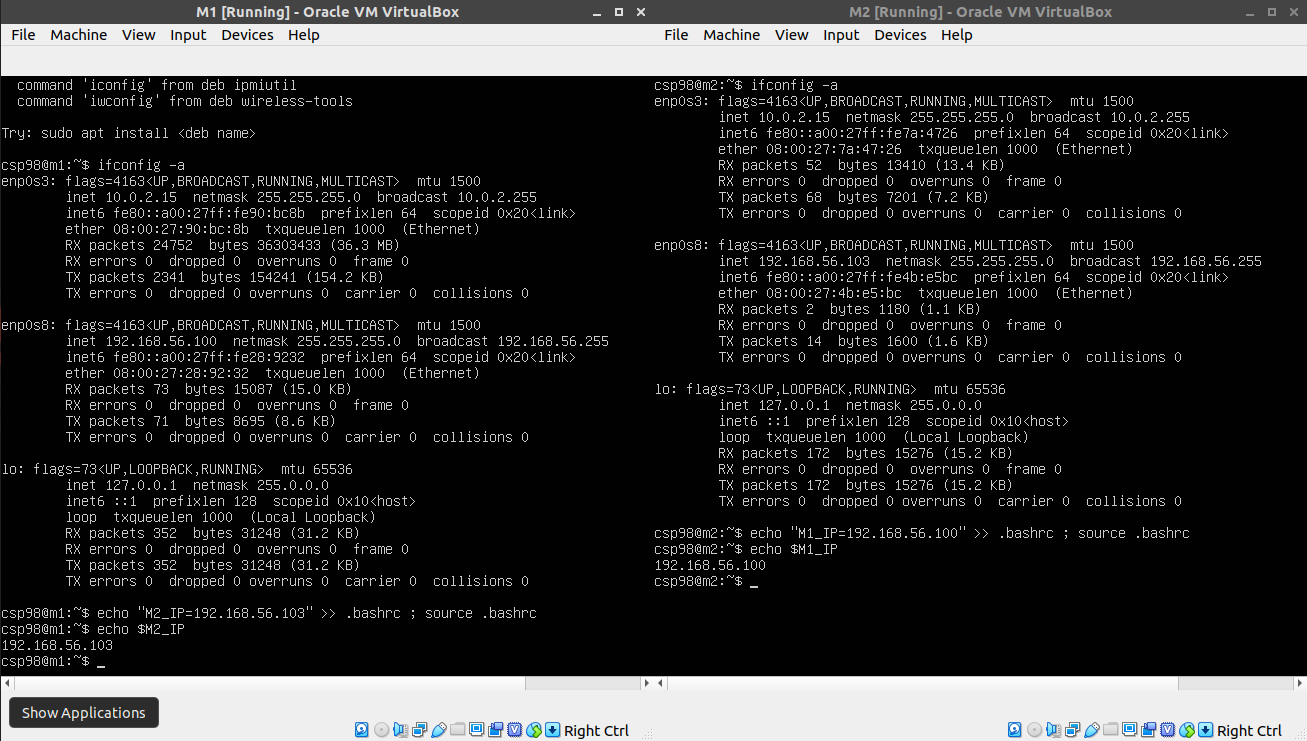
\includegraphics[scale=0.5]{/p1/ip_variable.png}
	\end{figure}
	\begin{figure}[H]
		\centering
		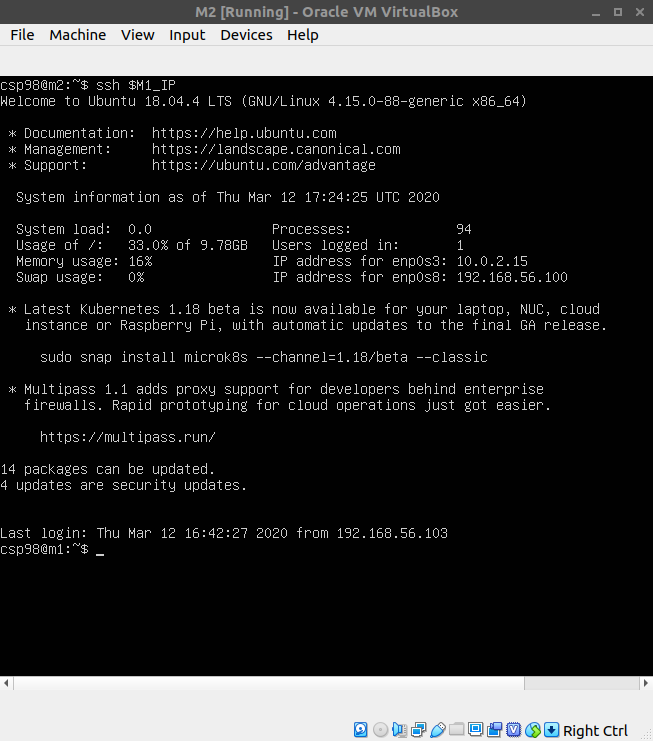
\includegraphics[scale=0.5]{/p1/ssh_ok.png}
	\end{figure}
	\item Creamos en \emph{M2} un documento HTML (\emph{/var/www/html/ejemplo.html}) con el siguiente contenido:
	\begin{lstlisting}
		<HTML>
		<BODY>
		Web de ejemplo de <nombre usuario> para SWAP
		</BODY>
		</HTML>
	\end{lstlisting}
	\item Hacemos \emph{curl} desde la otra máquina y comprobamos que recibimos la respuesta esperada:
	\begin{figure}[H]
		\centering
		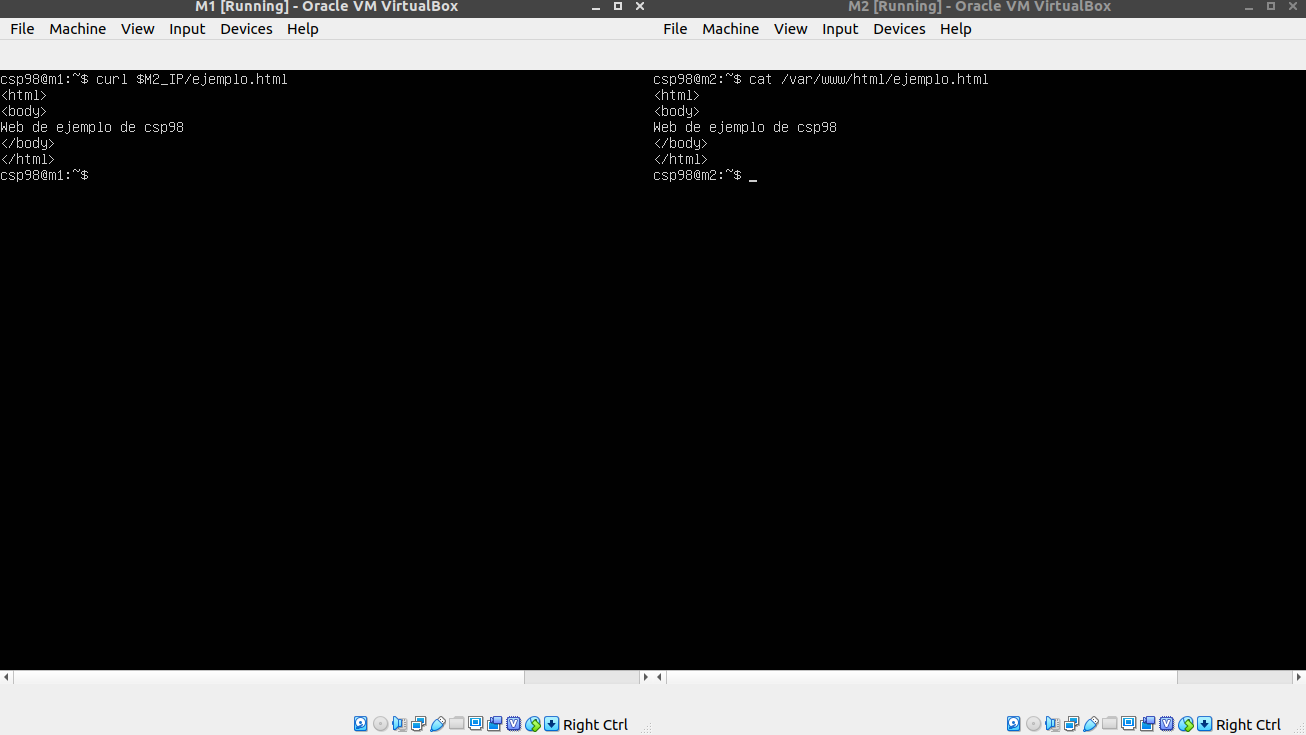
\includegraphics[scale=0.65]{/p1/curl_ok.png}
	\end{figure}
\end{enumerate}




\end{document}
